\documentclass[10pt]{article}
\usepackage{cacs2026}
\usepackage{amsmath}
\usepackage{multirow}
\usepackage{tikz}
\usetikzlibrary{arrows.meta,positioning,calc}
\usepackage{pgfplots}
\pgfplotsset{compat=1.18}

% Allow several small tables to stack at the top of one page instead of
% being forced onto a float-only page.
\setcounter{topnumber}{4}
\setcounter{totalnumber}{6}
\renewcommand{\topfraction}{0.95}
\renewcommand{\textfraction}{0.03}
\renewcommand{\floatpagefraction}{0.9}

% Colorblind-safe series colors shared by the figures.
\definecolor{vizblue}{HTML}{2A78D6}   % StreamVGGT
\definecolor{vizorange}{HTML}{EB6834} % Evict3R
\definecolor{vizaqua}{HTML}{1BAF7A}   % InfiniteVGGT
\definecolor{vizviolet}{HTML}{4A3AA7} % Keep3R (ours)

% -----------------------------------------------------------------------------
% CACS 2026 submission
% Compile with: latexmk -pdf main.tex
% Page budget: <= 6.5 pages including references (final target: 6 pages).
% -----------------------------------------------------------------------------

% Method name -- change here to rename globally.
\newcommand{\method}{Keep3R}

\begin{document}

\CACSmaketitle
  {\method: Memory-Bounded Streaming Visual Geometry\\ for Long-Horizon Robotic Manipulation}
  {First A. Author, Second B. Author, and Third C. Author
   % TODO(authors): fill in real author list and IEEE membership notes.
  }

\begin{CACSabstract}
\abstractnameCACS Robotic manipulation requires continual visual geometry perception, in which camera poses, per-pixel depth, and dense 3D structure of the workspace must be maintained from a single camera stream over hundreds of frames. Visual geometry foundation models provide strong geometric priors but operate offline, and their causal streaming variants accumulate a key--value (KV) cache whose memory and attention cost grow linearly with sequence length. We present \method{}, a training-free cache-management framework that bounds this growth with a fixed token budget by retaining the historical tokens that later viewpoints actually depend on. Cross-frame attention saliency measures this dependence, spatial smoothing and temporal aggregation stabilize it, and a budgeted compression step fuses it with a feature-diversity score under per-layer allocation, while reference-frame anchoring preserves the global coordinate frame. On single-camera DROID manipulation streams with PointWorld-DROID annotations, \method{} matches the reconstruction quality of the strongest streaming baselines while running about twice as fast and keeping peak VRAM near 9.5\,GB from 100 to 500 frames, whereas the full-cache backbone runs out of memory at 300 frames on a 48\,GB GPU. Geometry quality varies by at most 1.1\% over a $16\times$ budget range, so the budget acts as a pure deployment cost knob.

\end{CACSabstract}

\CACSfirstpagefootnote{%
% TODO(authors): replace with real support acknowledgment and affiliations.
This work was supported by [funding agency placeholder].\\
F. A. Author is with the Department of [Placeholder], [University Placeholder],
Taipei, Taiwan (e-mail: author@placeholder.edu.tw).\\
S. B. Author and T. C. Author are with [University Placeholder], Taiwan
(e-mail: \{author2, author3\}@placeholder.edu.tw).}

\section{Introduction}
\label{sec:intro}

Robotic manipulation demands \emph{continual} visual perception. To grasp, place, and rearrange objects, a robot needs camera poses, per-pixel depth, and dense 3D structure of its workspace at every step of an episode spanning hundreds of frames, often from a single camera. These estimates must also remain consistent in one coordinate frame to be useful for planning and control. Classical pipelines built on feature matching and bundle adjustment~\cite{schonberger2016sfm} handle textured, static scenes well but degrade under the weak textures, reflective surfaces, and persistent occlusions typical of manipulation.

Visual geometry foundation models replace hand-crafted geometric pipelines with learned priors. DUSt3R~\cite{wang2024dust3r} regresses dense pointmaps directly from image pairs without known intrinsics, VGGT~\cite{wang2025vggt} predicts cameras, depth, and pointmaps for many views in a single all-to-all forward pass, and Fast3R~\cite{yang2025fast3r} scales such inference to over a thousand images. All of these, however, consume images as a batch. StreamVGGT~\cite{zhuo2025streamvggt} instead processes each incoming frame exactly once while attending to a key--value (KV) cache of all past tokens, matching the frame-by-frame arrival of robot observations. The cache, however, grows linearly with time, and the full-cache backbone exhausts a 48\,GB GPU at 300 frames in our experiments (Table~\ref{tab:efficiency}).

Bounding the cache is therefore not optional; the question is what to keep. Manipulation streams have a particular structure, in which a static workspace of table surfaces, fixtures, and background is revisited by later viewpoints throughout the episode while the gripper and manipulated objects are transient, so evicting by recency or at random discards exactly the long-lived references that keep late frames registered to the workspace. KV-cache eviction is well studied for language models~\cite{zhang2023h2o,xiao2024streamingllm}, but language tokens live on a one-dimensional sequence, whereas visual geometry tokens carry both a 2D image position and a 3D interpretation, and selecting them independently fragments the local context on which dense prediction heads rely.

We therefore present \method{}, a training-free, fixed-budget cache-management framework built on a causal streaming visual geometry backbone (Fig.~\ref{fig:pipeline}). \method{} scores every cached token by cross-frame attention saliency (CFAS), the attention mass it receives from the current frame, which directly measures whether later viewpoints still depend on it. Spatial coherence regularization (SCR) smooths these scores over each source frame's patch grid, temporal saliency aggregation (TSA) accumulates them across time to suppress single-frame noise, and budgeted cache compression (BCC) fuses the result with a feature-diversity score to select the surviving tokens under a fixed total budget $B$ with per-layer allocation, while reference-frame anchoring pins the first frame, which defines the global coordinate frame. We evaluate on single-camera DROID~\cite{khazatsky2024droid} manipulation streams from both wrist-view and third-person cameras, using the geometry annotations of PointWorld-DROID~\cite{huang2026pointworld} as reference, and compare with recurrent-state methods (CUT3R~\cite{wang2025cut3r}, TTT3R~\cite{chen2025ttt3r}), the full-cache backbone StreamVGGT~\cite{zhuo2025streamvggt}, and memory-bounded streaming methods (Evict3R~\cite{mahdi2025evict3r}, InfiniteVGGT~\cite{yuan2026infinitevggt}). \method{} matches the reconstruction quality of the strongest baselines in every setting they complete, runs about twice as fast as the best memory-bounded alternative, and holds peak VRAM near 9.5\,GB from 100 to 500 frames.

Our contributions are as follows:
\begin{itemize}
\item We propose a fixed-budget streaming visual geometry framework for long-horizon single-camera manipulation streams, whose memory footprint and per-step attention cost are bounded by a token budget rather than by sequence length.
\item We design an attention-guided cache-retention mechanism that measures cross-frame dependence, regularizes it spatially and temporally, and fuses it with feature diversity under budgeted per-layer allocation with reference-frame anchoring.
\item We establish a manipulation-centric evaluation protocol on DROID streams of up to 500 frames, comparing against five streaming and online baselines with extensive ablations. \method{} attains on-par geometry at about twice the throughput of prior memory-bounded methods, and its quality varies by at most 1.1\% across a $16\times$ budget range.
\end{itemize}

\section{Related Work}
\label{sec:related}

\subsection{Visual Geometry Foundation Models}
DUSt3R~\cite{wang2024dust3r} reformulates 3D reconstruction as pointmap regression, mapping an image pair directly to dense 3D points in a shared coordinate frame without known intrinsics or poses, and MASt3R~\cite{leroy2024mast3r} grounds image matching in the same representation. Because pairwise inference must be followed by global alignment, cost grows rapidly with the number of views. Fast3R~\cite{yang2025fast3r} removes the pairwise bottleneck by reconstructing more than a thousand images in one forward pass, and VGGT~\cite{wang2025vggt} predicts cameras, depth maps, pointmaps, and point tracks with a single feed-forward transformer attending over all views. These models assume that a batch of images is available in advance, and all-to-all attention bounds the number of views that fit in memory, whereas a robot receives frames one at a time and cannot wait for the episode to end.

\subsection{Streaming and Online 3D Reconstruction}
Spann3R~\cite{wang2025spann3r} extends pointmap regression with an external spatial memory that is queried and updated frame by frame, and Point3R~\cite{wu2025point3r} maintains an explicit spatial pointer memory anchored in 3D space. CUT3R~\cite{wang2025cut3r} and TTT3R~\cite{chen2025ttt3r} instead compress history into a fixed-size recurrent state, which bounds cost by construction but forces all past geometry through a single lossy state, and LONG3R~\cite{chen2025long3r} sustains long streams by filtering a spatio-temporal memory. StreamVGGT~\cite{zhuo2025streamvggt} re-trains VGGT with causal attention and caches the keys and values of every past frame, preserving token-level geometric detail at the price of a cache that grows without bound. Our work keeps the token-level cache, and the quality that comes with it, while bounding its size. DROID~\cite{khazatsky2024droid} supplies exactly the long single-camera episodes this setting targets, and 3D world models such as PointWorld~\cite{huang2026pointworld} presuppose the reliable scene geometry we aim to provide.

\subsection{KV-Cache Compression and Token Eviction}
For language models, H$_2$O~\cite{zhang2023h2o} retains heavy-hitter tokens ranked by accumulated attention, and StreamingLLM~\cite{xiao2024streamingllm} keeps initial attention-sink tokens plus a sliding window. Within single images, token merging methods such as ToMe~\cite{bolya2023tome} reduce vision transformer cost. All of these treat tokens as independent sequence elements. For streaming geometry transformers, Evict3R~\cite{mahdi2025evict3r} evicts redundant tokens without any training, InfiniteVGGT~\cite{yuan2026infinitevggt} manages the cache for endless streams, FastVGGT~\cite{wang2026fastvggt} merges near-duplicate tokens to accelerate inference, and GHOST~\cite{chen2026ghost} drives eviction with the model's own geometry outputs. All target generic video streams and rank tokens by importance, redundancy, or predicted geometry alone. \method{} differs in coupling cross-frame dependence with spatial coherence, temporal stability, and a diversity-balanced per-layer budget under one fixed total allocation, and in targeting manipulation streams, where a revisited static workspace and a transient dynamic foreground make retention decisions consequential.

\section{Method}
\label{sec:method}

\begin{figure*}[t]
    \centering
    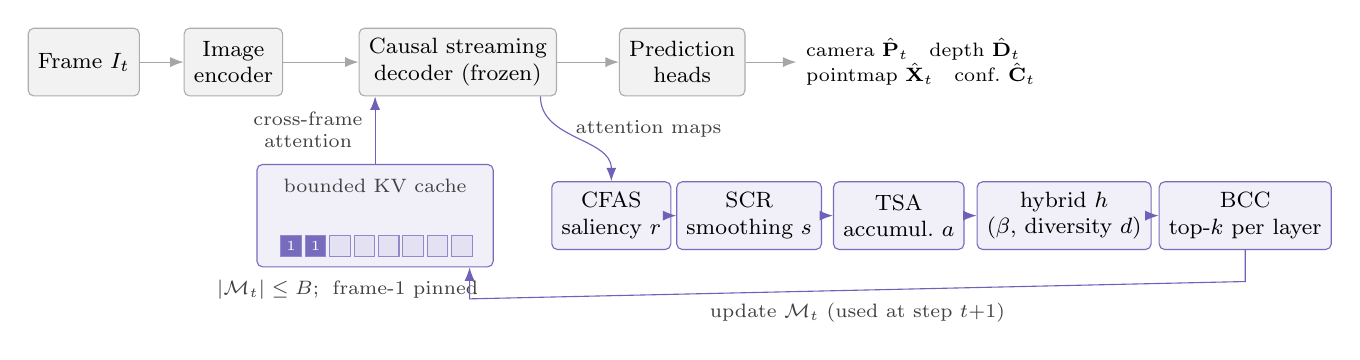
\begin{tikzpicture}[
        font=\footnotesize,
        >={Latex[length=1.7mm]},
        bb/.style={draw=gray!65, fill=gray!10, rounded corners=2pt,
                   minimum height=0.86cm, align=center, inner sep=3.5pt},
        cpath/.style={draw=vizviolet!75, fill=vizviolet!8, rounded corners=2pt,
                   minimum height=0.86cm, align=center, inner sep=3.5pt},
        lbl/.style={font=\scriptsize, text=black!75, align=center},
    ]
        % Backbone lane.
        \node[bb] (frame) at (0.6,0) {Frame $I_t$};
        \node[bb] (enc)   at (2.5,0) {Image\\encoder};
        \node[bb] (dec)   at (5.35,0) {Causal streaming\\decoder (frozen)};
        \node[bb] (heads) at (8.2,0) {Prediction\\heads};
        \node[anchor=west, align=left, font=\scriptsize] (out) at (9.65,0)
            {camera $\hat{\mathbf{P}}_t$ \; depth $\hat{\mathbf{D}}_t$\\
             pointmap $\hat{\mathbf{X}}_t$ \; conf.\ $\hat{\mathbf{C}}_t$};
        \draw[->, gray!70] (frame) -- (enc);
        \draw[->, gray!70] (enc) -- (dec);
        \draw[->, gray!70] (dec) -- (heads);
        \draw[->, gray!70] (heads) -- (out.west);
        % Bounded cache with pinned frame-1 cells.
        \node[cpath, minimum width=3.0cm, minimum height=1.3cm] (cache) at (4.3,-1.95)
            {};
        \node[lbl, anchor=north] at ([yshift=-2pt]cache.north) {bounded KV cache};
        \foreach \i/\c in {0/vizviolet!75, 1/vizviolet!75, 2/vizviolet!15,
                           3/vizviolet!15, 4/vizviolet!15, 5/vizviolet!15,
                           6/vizviolet!15, 7/vizviolet!15}{
            \draw[draw=vizviolet!60, fill=\c]
                ($(cache.south west)+(0.31+0.31*\i,0.14)$) rectangle ++(0.26,0.26);}
        \node[font=\tiny, text=white] at ($(cache.south west)+(0.44,0.27)$) {1};
        \node[font=\tiny, text=white] at ($(cache.south west)+(0.75,0.27)$) {1};
        \node[lbl, anchor=north] at ([xshift=-0.35cm,yshift=-1pt]cache.south)
            {$|\mathcal{M}_t|\le B$;\; frame-1 pinned};
        % Cache-scoring chain.
        \node[cpath] (cfas) at (7.3,-1.95)  {CFAS\\saliency $r$};
        \node[cpath] (scr)  at (9.05,-1.95) {SCR\\smoothing $s$};
        \node[cpath] (tsa)  at (10.95,-1.95) {TSA\\accumul.\ $a$};
        \node[cpath] (mix)  at (13.05,-1.95) {hybrid $h$\\($\beta$, diversity $d$)};
        \node[cpath] (bcc)  at (15.35,-1.95) {BCC\\top-$k$ per layer};
        \draw[->, vizviolet!80] (cfas) -- (scr);
        \draw[->, vizviolet!80] (scr) -- (tsa);
        \draw[->, vizviolet!80] (tsa) -- (mix);
        \draw[->, vizviolet!80] (mix) -- (bcc);
        % Cache <-> decoder and update loop.
        \draw[->, vizviolet!80] (cache.north) --
            node[lbl, left=1pt] {cross-frame\\attention}
            (cache.north |- dec.south);
        \draw[->, vizviolet!80] ([xshift=1.05cm]dec.south) to[out=-90, in=90]
            node[lbl, pos=0.35, right=2pt] {attention maps} (cfas.north);
        \draw[->, vizviolet!80] (bcc.south) -- ++(0,-0.4) --
            node[lbl, below=1pt] {update $\mathcal{M}_t$ (used at step $t{+}1$)}
            ($(cache.south)+(1.2,-0.4)$) -- ([xshift=1.2cm]cache.south);
    \end{tikzpicture}
    \caption{Overview of \method. Each incoming frame is encoded and decoded causally against a bounded KV cache, yielding per-frame camera parameters, depth, pointmap, and confidence. The cross-frame attention of the current frame provides a saliency signal for every cached token (CFAS), which is smoothed over the source patch grid (SCR) and accumulated over time (TSA). Budgeted cache compression (BCC) fuses the accumulated importance with a diversity score, allocates the budget across layers, and retains the top-scoring tokens, with the reference frame pinned, so that the cache never exceeds $B$ tokens.}
    \label{fig:pipeline}
\end{figure*}

\method\ turns a causal streaming visual geometry transformer into a fixed-memory continual perception system. Given a monocular manipulation stream, it outputs camera parameters, depth, and a dense pointmap for every incoming frame, while a budgeted cache-management mechanism decides which historical tokens remain visible to future frames.

\subsection{Problem Formulation}
\label{sec:formulation}

We consider a monocular RGB stream $\mathcal{I}=\{I_t\}_{t=1}^{T}$ captured during a robotic manipulation episode. At step $t$ the model observes only the current frame and a bounded cache $\mathcal{M}_{t-1}$ of historical KV tokens, and predicts
\begin{equation}
(\hat{\mathbf{P}}_t, \hat{\mathbf{D}}_t, \hat{\mathbf{X}}_t, \hat{\mathbf{C}}_t)
= f_{\theta}(I_t, \mathcal{M}_{t-1}),
\label{eq:streaming}
\end{equation}
where $\hat{\mathbf{P}}_t=(\hat{\mathbf{K}}_t, \hat{\mathbf{T}}_t)$ contains the camera intrinsics and the camera-to-world pose $\hat{\mathbf{T}}_t\in\mathrm{SE}(3)$, $\hat{\mathbf{D}}_t$ is a per-pixel depth map, $\hat{\mathbf{X}}_t$ is a dense 3D pointmap in the camera coordinates of frame $t$, and $\hat{\mathbf{C}}_t$ is the associated confidence map. We instantiate $f_{\theta}$ with a frozen causal streaming visual geometry transformer~\cite{zhuo2025streamvggt}, which encodes each frame into patch tokens and a few auxiliary tokens~\cite{dosovitskiy2021vit,wang2025vggt} and lets the tokens of frame $t$ attend to the cached KV tokens of all earlier frames~\cite{vaswani2017attention}.

Let $\mathcal{Z}_t^{\ell}$ denote the tokens frame $t$ contributes to decoder layer $\ell\in\{1,\dots,L\}$, with $N_t^{\ell}=|\mathcal{Z}_t^{\ell}|$, and let $\mathcal{M}_t$ be the union of the per-layer caches $\mathcal{M}_t^{\ell}$. If every token is kept, the cache grows by $\sum_{\ell} N_t^{\ell}$ tokens per frame, so memory and per-step attention cost increase linearly and without bound, and for manipulation episodes of hundreds of frames this growth is the dominant deployment bottleneck.

\method\ instead maintains $|\mathcal{M}_t|\le B$ for a fixed token budget $B$ by selecting, at every step and layer, a retained set $\mathcal{R}_t^{\ell}$ from the cached and newly produced tokens. Ideally, retention should preserve the behavior of the unbounded model,
\begin{equation}
\begin{aligned}
\min_{\{\mathcal{R}_t^{\ell}\}}\;
& \sum_{t=1}^{T}
\mathcal{L}\!\left(
f^{\mathrm{geo}}_{\theta}(I_t, \mathcal{M}_{t-1}),\,
f^{\mathrm{geo}}_{\theta}(I_t, \mathcal{M}^{\mathrm{full}}_{t-1})
\right) \\
\text{s.t.}\;
& \sum\nolimits_{\ell=1}^{L} |\mathcal{R}_t^{\ell}| \le B,
\qquad \forall t,
\end{aligned}
\label{eq:objective}
\end{equation}
where $\mathcal{M}^{\mathrm{full}}_{t-1}$ is the unbounded cache, $f^{\mathrm{geo}}_{\theta}$ denotes the camera, depth, and pointmap outputs, and $\mathcal{L}$ is any discrepancy between them. Objective~\eqref{eq:objective} cannot be optimized online, because evaluating the full-cache reference requires exactly the memory we aim to bound, and the effect of evicting a token depends on frames that have not yet arrived. \method\ therefore uses the attention that later frames direct at a cached token as a streaming surrogate for its contribution to~\eqref{eq:objective}, since a token that current queries keep consulting is one whose eviction would perturb future predictions the most.

\subsection{Cross-Frame Attention Saliency}
\label{sec:cfas}

In the causal decoder, current-frame queries retrieve geometric context from the cache through cross-frame attention. Let $\mathbf{A}^{\ell,h}_{t}\in\mathbb{R}^{N_t^{\ell}\times|\mathcal{M}^{\ell}_{t-1}|}$ be the attention matrix from the layer-$\ell$ queries of frame $t$ to the cached layer-$\ell$ tokens in head $h$. CFAS defines the saliency of cached token $i$ as the attention mass it receives, averaged over the $H$ heads and $N_t^{\ell}$ queries:
\begin{equation}
r^{\ell}_{t,i}
= \frac{1}{H}\sum_{h=1}^{H}\frac{1}{N_t^{\ell}}
\sum_{j=1}^{N_t^{\ell}}
\bigl[\mathbf{A}^{\ell,h}_{t}\bigr]_{j,i}.
\label{eq:cfas}
\end{equation}
CFAS measures view dependence rather than local distinctiveness. It is high not for tokens that were salient in their source image, but for tokens the model actively consults from the current viewpoint when reasoning about geometry. In manipulation streams these are typically tokens of repeatedly revisited static workspace structure, whereas tokens covering transient foreground receive little attention once the gripper has moved on. The next two components adapt this signal to visual geometry tokens, which, unlike language tokens, carry 2D image-space and 3D scene structure.

\subsection{Spatial Coherence Regularization}
\label{sec:scr}

Selecting tokens by $r^{\ell}_{t,i}$ alone produces spatially fragmented caches. Patch tokens tile the image plane, adjacent tokens usually cover the same physical surface, and the dense prediction heads rely on local context, so a cache of isolated survivors degrades depth and pointmap continuity. SCR therefore smooths saliency over the source-frame patch grid. For each source frame $\tau<t$ still represented in the layer-$\ell$ cache, we scatter the scores of its cached patch tokens back onto its patch grid, obtaining a score map $\mathbf{R}^{\ell}_{t,\tau}$ with vacant positions set to zero, and blend it with a Gaussian-filtered copy:
\begin{equation}
\widetilde{\mathbf{R}}^{\ell}_{t,\tau}
= (1-\alpha)\,\mathbf{R}^{\ell}_{t,\tau}
+ \alpha\,\mathcal{G}_{\sigma}\bigl(\mathbf{R}^{\ell}_{t,\tau}\bigr),
\qquad \alpha\in[0,1],
\label{eq:scr_blend}
\end{equation}
where $\mathcal{G}_{\sigma}$ is a Gaussian filter with scale $\sigma$ and $\alpha$ controls the smoothing strength. Each patch token then reads its smoothed score $s^{\ell}_{t,i}=\widetilde{\mathbf{R}}^{\ell}_{t,t_i}[\mathbf{u}_i]$ at its source frame $t_i$ and source position $\mathbf{u}_i$, while auxiliary tokens, which have no grid position, keep their raw scores $s^{\ell}_{t,i}=r^{\ell}_{t,i}$. SCR does not alter the network's predictions; it only biases retention toward spatially coherent regions, which suits workspace geometry that appears as contiguous surfaces rather than isolated patches.

\subsection{Temporal Saliency Aggregation}
\label{sec:tsa}

Single-step saliency is noisy, since a token that matters over the long term may receive little attention in one frame because of occlusion, motion blur, or attention fluctuation, while a token noticed once may never be needed again. TSA accumulates saliency with an exponential moving sum,
\begin{equation}
a^{\ell}_{t,i} =
\begin{cases}
\gamma\, a^{\ell}_{t-1,i} + s^{\ell}_{t,i}, & i\in\mathcal{M}^{\ell}_{t-1},\\[2pt]
a_{\mathrm{init}}, & i\in\mathcal{Z}^{\ell}_{t},
\end{cases}
\label{eq:tsa}
\end{equation}
where $\gamma\in[0,1]$ controls how long past evidence persists, and new tokens enter with a fixed score $a_{\mathrm{init}}$ because no later frame has queried them yet. Accumulators of evicted tokens are discarded. TSA separates tokens that are persistently relied upon from tokens that were attended only briefly, which is precisely the distinction between static workspace structure and transient foreground.

\subsection{Budgeted Cache Compression}
\label{sec:bcc}

After the forward pass of frame $t$, BCC reduces the layer-$\ell$ candidate set $\mathcal{C}^{\ell}_{t}=\mathcal{M}^{\ell}_{t-1}\cup\mathcal{Z}^{\ell}_{t}$ to the retained set $\mathcal{R}^{\ell}_{t}$ under the global budget $B$. Importance alone would repeatedly select near-duplicate tokens of the most-attended surfaces, so BCC balances it against representational diversity $d^{\ell}_{t,i} = 1 - \cos(\mathbf{k}^{\ell}_{i}, \bar{\mathbf{k}}^{\ell}_{t})$, the cosine distance of token $i$'s key to the mean key $\bar{\mathbf{k}}^{\ell}_{t}$ of the candidate set, which is large for tokens carrying rare geometric evidence. Because importance and diversity live on different scales, both are min--max normalized within the layer-$\ell$ candidate set (operator $\operatorname{Norm}^{\ell}_{t}$; a small $\epsilon$ guards the denominator) and fused into the hybrid retention score
\begin{equation}
h^{\ell}_{t,i}
= \beta \operatorname{Norm}^{\ell}_{t}\!\bigl(a^{\ell}_{t,i}\bigr)
+ (1-\beta)\operatorname{Norm}^{\ell}_{t}\!\bigl(d^{\ell}_{t,i}\bigr),
\label{eq:hybrid}
\end{equation}
where $\beta\in[0,1]$ trades importance against diversity.

The budget is distributed across layers in proportion to their mean diversity $D^{\ell}_{t}=\frac{1}{|\mathcal{C}^{\ell}_{t}|}\sum_{i} d^{\ell}_{t,i}$, so layers with more heterogeneous candidates receive more slots:
\begin{equation}
\widetilde{B}^{\ell}_{t}
= \Bigl\lfloor
B^{\mathrm{free}}\,
\frac{D^{\ell}_{t}}{\sum_{m=1}^{L} D^{m}_{t}}
\Bigr\rfloor,
\qquad
B^{\mathrm{free}} = B - \sum\nolimits_{\ell} |\mathcal{Z}^{\ell}_{1}|,
\label{eq:allocation}
\end{equation}
where $B^{\mathrm{free}}$ is the budget left after reserving the anchored first frame (below). Slots lost to rounding are redistributed to the layers with the largest fractional remainders, and if all diversities vanish the free budget is split equally. Each layer then keeps its top-scoring candidates,
\begin{equation}
\mathcal{R}^{\ell}_{t}
= \mathcal{Z}^{\ell}_{1} \cup
\operatorname{TopK}_{\widetilde{B}^{\ell}_{t}}\!
\bigl(\mathcal{C}^{\ell}_{t}\setminus\mathcal{Z}^{\ell}_{1};\, h^{\ell}_{t}\bigr),
\label{eq:retention}
\end{equation}
where $\operatorname{TopK}_{n}(\cdot\,;h)$ returns the $\min(n,|\cdot|)$ candidates with the highest hybrid scores, and the updated cache is $\mathcal{M}^{\ell}_{t}=\mathcal{R}^{\ell}_{t}$. At $t{=}1$ there is no history, so the cache is initialized with all frame-1 tokens and every accumulator starts at $a_{\mathrm{init}}$.

\textit{Reference-frame anchoring.} The causal backbone expresses all geometry in the coordinate frame of the first frame~\cite{zhuo2025streamvggt}, so the tokens of frame 1 act as the global reference against which every later prediction is aligned. \method\ pins them, excluding them from the top-$K$ selection so they are never evicted, a role analogous to the attention sinks that stabilize streaming language models~\cite{xiao2024streamingllm}. A single frame contributes $|\mathcal{Z}_1|\ll B$ tokens, so the pinned set occupies a small, constant fraction of the budget.

Together, these components keep $|\mathcal{M}_t|\le B$ at every step, so cache memory and per-step attention cost are $O(B)$ regardless of $T$, and the whole mechanism is training-free, adding only score maps and scalar accumulators on top of quantities the backbone already computes.

\section{Experiments}
\label{sec:experiments}

We evaluate \method{} on geometric quality (depth and dense reconstruction), on inference efficiency (throughput and memory), and through ablations of the retention mechanism itself. All methods process identical frame sequences in a strictly causal, frame-by-frame fashion without access to future frames.

\subsection{Experimental Setup}
\label{sec:exp-setup}

\textit{Data.}
We build our benchmark from DROID~\cite{khazatsky2024droid}, a large-scale in-the-wild robot manipulation dataset. From each episode we extract two single-camera stream types, namely a \emph{wrist-view} (WV) stream with strong ego-motion and close-range dynamic foreground, and a \emph{third-person} (TP) stream from a static external camera observing the full workspace. For each view type we evaluate three sequence lengths $T\in\{100,300,500\}$ with five episodes per setting; episodes shorter than the target length are excluded.
% TODO(rerun): confirm the final episode list used for the camera-ready runs.
% TODO(verify): confirm the official name of the PointWorld label release for DROID
% (the PointWorld abstract does not mention DROID explicitly; verify against the
% paper body / released assets that "PointWorld-DROID" is the correct designation).
As reference geometry we use the per-frame depth, camera, and pointmap annotations of PointWorld-DROID~\cite{huang2026pointworld}; since these labels are model-generated rather than sensor-measured, we account for this when interpreting absolute errors.

\textit{Metrics.}
Depth quality is measured per frame by the absolute relative error
$\mathrm{AbsRel}=\frac{1}{|\Omega|}\sum_{\mathbf{p}\in\Omega}|\hat{D}(\mathbf{p})-D(\mathbf{p})|/D(\mathbf{p})$
and the threshold accuracy $\delta{<}1.25$, the fraction of pixels in the valid set $\Omega$ with $\max(\hat{D}/D,\,D/\hat{D})<1.25$~\cite{eigen2014depth}.
Reconstruction quality compares predicted pointmaps against the reference pointmaps using Accuracy (distance from each predicted point to its nearest reference point, in meters), Completeness (the reverse direction), and Normal Consistency (NC)~\cite{yao2018mvsnet}; we report means and medians, which differ noticeably in the presence of outlier regions. Efficiency is measured by end-to-end throughput (FPS) and peak VRAM on a single GPU, together with whether a method completes all sequences without running out of memory (OOM).

\textit{Baselines.}
CUT3R~\cite{wang2025cut3r} and TTT3R~\cite{chen2025ttt3r} compress history into a fixed-size recurrent state. StreamVGGT~\cite{zhuo2025streamvggt} is the causal streaming backbone with an unbounded full KV cache. Evict3R~\cite{mahdi2025evict3r} performs training-free token eviction on streaming visual geometry transformers, and InfiniteVGGT~\cite{yuan2026infinitevggt} manages the cache of VGGT-style models for endless streams; these two are the most direct memory-bounded baselines.

\textit{Implementation.}
\method{} is training-free and plugs into frozen StreamVGGT weights. Unless stated otherwise, we use a total budget $B{=}200\mathrm{k}$ tokens, SCR strength $\alpha=0.5$, TSA decay $\gamma=0.9$, and mixing weight $\beta=0.5$.
% TODO(rerun): confirm the a_init value used in the final runs and state it here.
All methods run on one NVIDIA RTX 6000 Ada GPU (48\,GB) with PyTorch 2.9 and CUDA 12.8.

\subsection{Depth Estimation}
\label{sec:exp-depth}

% TODO(rerun): all "Ours" rows in this section were produced by the thesis configuration; re-run with the final method (no workspace anchors / DFS) and update. Changes are expected to be within noise.
\begin{table}[t]
    \centering
    \caption{Depth estimation on DROID manipulation streams. Each cell reports $T{=}100/300/500$; bold marks the best among methods that complete all sequence lengths.}
    \label{tab:depth}
    \tabletext
    \setlength{\tabcolsep}{3pt}
    \begin{tabular}{clcc}
        \toprule
        View & Method & Abs Rel $\downarrow$ & $\delta{<}1.25$ $\uparrow$ \\
        \midrule
        \multirow{6}{*}{TP}
        & CUT3R~\cite{wang2025cut3r}                & 0.637/0.625/0.614 & 0.306/0.307/0.306 \\
        & TTT3R~\cite{chen2025ttt3r}                & \textbf{0.635}/\textbf{0.621}/\textbf{0.610} & \textbf{0.311}/\textbf{0.315}/\textbf{0.314} \\
        & StreamVGGT~\cite{zhuo2025streamvggt}      & 0.652/OOM/OOM     & 0.297/OOM/OOM \\
        & Evict3R~\cite{mahdi2025evict3r}           & 0.650/0.636/0.624 & 0.295/0.297/0.297 \\
        & InfiniteVGGT~\cite{yuan2026infinitevggt}  & 0.652/0.638/0.628 & 0.296/0.301/0.300 \\
        & \method{} (ours)                          & 0.650/0.633/0.623 & 0.296/0.302/0.301 \\
        \midrule
        \multirow{6}{*}{WV}
        & CUT3R~\cite{wang2025cut3r}                & 0.514/0.798/0.710 & 0.512/0.451/0.459 \\
        & TTT3R~\cite{chen2025ttt3r}                & 0.513/0.788/0.706 & 0.510/0.450/0.456 \\
        & StreamVGGT~\cite{zhuo2025streamvggt}      & 0.407/OOM/OOM     & 0.515/OOM/OOM \\
        & Evict3R~\cite{mahdi2025evict3r}           & 0.415/0.662/0.600 & 0.512/0.450/\textbf{0.460} \\
        & InfiniteVGGT~\cite{yuan2026infinitevggt}  & \textbf{0.408}/0.658/\textbf{0.597} & \textbf{0.515}/\textbf{0.452}/\textbf{0.460} \\
        & \method{} (ours)                          & 0.413/\textbf{0.657}/\textbf{0.597} & 0.511/0.447/0.456 \\
        \bottomrule
    \end{tabular}
\end{table}

Table~\ref{tab:depth} reports depth results, with two patterns. First, the recurrent-state methods lead on the third-person stream, where TTT3R attains the lowest AbsRel at every length, but degrade sharply on the wrist-view stream once sequences grow; at $T\geq300$ their WV AbsRel rises to $0.706$--$0.798$, whereas all cache-based methods remain near $0.60$--$0.66$, which suggests that a single compressed state is insufficient under the strong ego-motion of a wrist camera. Second, within the cache-based class the differences are small (within about 2\%), and \method{} attains the best or tied-best WV AbsRel at $T{=}300$ and $T{=}500$ while completing every setting. Depth quality does not deteriorate as sequences grow, and TP AbsRel in fact improves from $0.650$ at $T{=}100$ to $0.623$ at $T{=}500$, indicating that a fixed 200k-token cache preserves enough cross-frame context for stable long-horizon prediction.

\subsection{3D Reconstruction}
\label{sec:exp-recon}

\begin{table}[t]
    \centering
    \caption{3D reconstruction at $T{=}500$. Acc/Comp in meters (lower is better), NC higher is better; bold marks the best per column. Trends at $T{=}100$ and $T{=}300$ are consistent (see text).}
    \label{tab:recon}
    \tabletext
    \setlength{\tabcolsep}{2.6pt}
    \begin{tabular}{clcccccc}
        \toprule
        \multirow{2}{*}{View} & \multirow{2}{*}{Method}
        & \multicolumn{2}{c}{Acc.\ $\downarrow$}
        & \multicolumn{2}{c}{Comp.\ $\downarrow$}
        & \multicolumn{2}{c}{NC $\uparrow$} \\
        \cmidrule(lr){3-4}\cmidrule(lr){5-6}\cmidrule(lr){7-8}
        & & Mean & Med. & Mean & Med. & Mean & Med. \\
        \midrule
        \multirow{6}{*}{TP}
        & CUT3R~\cite{wang2025cut3r}               & 0.487 & 0.213 & \textbf{0.252} & 0.192 & 0.505 & 0.498 \\
        & TTT3R~\cite{chen2025ttt3r}               & 0.442 & 0.191 & 0.269 & 0.193 & \textbf{0.531} & \textbf{0.541} \\
        & StreamVGGT~\cite{zhuo2025streamvggt}     & OOM & OOM & OOM & OOM & OOM & OOM \\
        & Evict3R~\cite{mahdi2025evict3r}          & 0.105 & 0.084 & 0.374 & \textbf{0.133} & 0.491 & 0.477 \\
        & InfiniteVGGT~\cite{yuan2026infinitevggt} & 0.112 & 0.087 & 0.370 & \textbf{0.133} & 0.503 & 0.499 \\
        & \method{} (ours)                         & \textbf{0.103} & \textbf{0.083} & 0.375 & \textbf{0.133} & 0.514 & 0.512 \\
        \midrule
        \multirow{6}{*}{WV}
        & CUT3R~\cite{wang2025cut3r}               & 0.355 & 0.307 & 0.310 & 0.231 & 0.511 & 0.516 \\
        & TTT3R~\cite{chen2025ttt3r}               & 0.278 & 0.249 & 0.383 & 0.307 & 0.496 & 0.495 \\
        & StreamVGGT~\cite{zhuo2025streamvggt}     & OOM & OOM & OOM & OOM & OOM & OOM \\
        & Evict3R~\cite{mahdi2025evict3r}          & 0.085 & 0.065 & 0.167 & 0.054 & \textbf{0.529} & \textbf{0.545} \\
        & InfiniteVGGT~\cite{yuan2026infinitevggt} & \textbf{0.078} & 0.059 & 0.180 & 0.067 & 0.528 & 0.542 \\
        & \method{} (ours)                         & 0.079 & \textbf{0.054} & \textbf{0.162} & \textbf{0.047} & 0.520 & 0.530 \\
        \bottomrule
    \end{tabular}
\end{table}

Table~\ref{tab:recon} reports reconstruction quality at the longest horizon, $T{=}500$. The gap between the two method classes is much larger here than for depth, with cache-based methods reaching a mean TP Accuracy of $0.103$--$0.112$\,m, roughly a quarter of the error of the recurrent-state methods ($0.442$--$0.487$\,m). The recurrent methods do achieve lower mean TP Completeness ($0.252$\,m for CUT3R versus $0.370$--$0.375$\,m), but at substantially worse accuracy, and the Completeness gap narrows considerably at the median ($0.192$ versus $0.133$\,m).

Among memory-bounded methods, \method{} attains the best mean and median Accuracy on TP ($0.103/0.083$\,m) and the best WV Completeness in both statistics ($0.162/0.047$\,m), with WV mean Accuracy ($0.079$\,m) within $0.001$\,m of the best (InfiniteVGGT). Evict3R attains the best WV normal consistency. Trends at shorter horizons are consistent. At $T{=}100$, where the full-cache backbone can still run, \method{} attains the best TP mean Accuracy ($0.108$\,m versus $0.116$\,m for StreamVGGT), and its WV median Completeness is the lowest at every length ($0.074/0.056/0.047$\,m).

\subsection{Efficiency and Long-Horizon Stability}
\label{sec:exp-efficiency}

\begin{table}[t]
    \centering
    \caption{Inference efficiency of cache-based methods. Each cell reports $T{=}100/300/500$; bold marks the best per column.}
    \label{tab:efficiency}
    \tabletext
    \setlength{\tabcolsep}{3pt}
    \begin{tabular}{clcc}
        \toprule
        View & Method & FPS $\uparrow$ & Peak VRAM (GB) $\downarrow$ \\
        \midrule
        \multirow{4}{*}{TP}
        & StreamVGGT~\cite{zhuo2025streamvggt}     & 5.02/OOM/OOM   & 23.76/OOM/OOM \\
        & Evict3R~\cite{mahdi2025evict3r}          & 4.36/4.00/4.03 & 10.65/11.45/11.81 \\
        & InfiniteVGGT~\cite{yuan2026infinitevggt} & 5.18/3.88/3.75 & 16.25/16.50/16.62 \\
        & \method{} (ours)                         & \textbf{9.10}/\textbf{7.38}/\textbf{7.79} & \textbf{9.16}/\textbf{9.41}/\textbf{9.52} \\
        \midrule
        \multirow{4}{*}{WV}
        & StreamVGGT~\cite{zhuo2025streamvggt}     & 4.89/OOM/OOM   & 23.76/OOM/OOM \\
        & Evict3R~\cite{mahdi2025evict3r}          & 4.15/4.04/4.06 & 10.65/11.46/11.82 \\
        & InfiniteVGGT~\cite{yuan2026infinitevggt} & 4.56/3.91/3.87 & 16.32/16.57/16.68 \\
        & \method{} (ours)                         & \textbf{9.71}/\textbf{9.50}/\textbf{9.40} & \textbf{9.14}/\textbf{9.39}/\textbf{9.50} \\
        \bottomrule
    \end{tabular}
\end{table}

\begin{figure}[t]
    \centering
    % Data identical to the TP rows of Table 3.
    \pgfplotsset{
        effpanel/.style={
            width=4.72cm, height=3.25cm,
            xtick={100,300,500}, xmin=40, xmax=560,
            ymajorgrids, grid style={gray!22},
            axis line style={gray!55},
            tick label style={font=\scriptsize},
            label style={font=\scriptsize},
            xlabel={Sequence length $T$},
            ylabel near ticks, xlabel near ticks,
            xlabel shift=-2pt, ylabel shift=-3pt,
            every axis plot/.append style={line width=0.9pt, mark size=1.7pt},
        }}
    \begin{tikzpicture}
    \begin{axis}[effpanel, name=vram,
        ylabel={Peak VRAM (GB)}, ymin=0, ymax=27,
        legend to name=effleg, legend columns=4,
        legend style={font=\scriptsize, draw=none,
            /tikz/every even column/.append style={column sep=2.5pt}},
    ]
        \addplot[vizblue, mark=square*] coordinates {(100,23.76)};
        \addlegendentry{StreamVGGT}
        \addplot[vizorange, mark=triangle*] coordinates {(100,10.65) (300,11.45) (500,11.81)};
        \addlegendentry{Evict3R}
        \addplot[vizaqua, mark=diamond*] coordinates {(100,16.25) (300,16.50) (500,16.62)};
        \addlegendentry{InfiniteVGGT}
        \addplot[vizviolet, mark=*] coordinates {(100,9.16) (300,9.41) (500,9.52)};
        \addlegendentry{\method{} (ours)}
        \node[font=\scriptsize, text=vizblue, anchor=north west]
            at (axis cs:120,24.8) {OOM at $T{=}300$};
    \end{axis}
    \begin{axis}[effpanel,
        at={(vram.outer east)}, anchor=outer west, xshift=1mm,
        ylabel={Throughput (FPS)}, ymin=0, ymax=11,
    ]
        \addplot[vizblue, mark=square*] coordinates {(100,5.02)};
        \addplot[vizorange, mark=triangle*] coordinates {(100,4.36) (300,4.00) (500,4.03)};
        \addplot[vizaqua, mark=diamond*] coordinates {(100,5.18) (300,3.88) (500,3.75)};
        \addplot[vizviolet, mark=*] coordinates {(100,9.10) (300,7.38) (500,7.79)};
    \end{axis}
    \end{tikzpicture}
    \par\vspace{2pt}
    \ref{effleg}
    \caption{Peak VRAM and throughput versus sequence length on the third-person stream. \method{} keeps peak VRAM nearly constant and sustains the highest throughput, while the full-cache StreamVGGT runs out of memory at the 300-frame setting.}
    \label{fig:efficiency}
\end{figure}

Table~\ref{tab:efficiency} and Fig.~\ref{fig:efficiency} summarize efficiency. The recurrent-state methods have constant cost by construction but substantially weaker reconstruction (Table~\ref{tab:recon}), so this comparison focuses on the cache-based class. \method{} is the fastest in every setting, delivering $1.8$--$2.3\times$ the throughput of Evict3R ($4.00$--$4.36$ FPS) and InfiniteVGGT ($3.75$--$5.18$ FPS). Peak memory stays within $9.14$--$9.52$\,GB across all settings; growing the WV stream from $100$ to $500$ frames adds only $0.36$\,GB, and throughput drops by just $3.2$\%. In contrast, StreamVGGT already needs $23.76$\,GB at $T{=}100$ and exhausts a 48\,GB GPU at $T{\geq}300$, and InfiniteVGGT uses $16.2$--$16.7$\,GB.

\subsection{Ablation Studies}
\label{sec:exp-ablation}

All ablations use $T{=}500$ with the base configuration $B{=}200\mathrm{k}$, $\alpha{=}0.5$, $\gamma{=}0.9$, $\beta{=}0.5$; each variant changes one factor at a time.

\begin{table}[t]
    \centering
    \caption{Cache retention strategies ($T{=}500$). Parentheses give the relative change with respect to \method{}; negative is worse.}
    \label{tab:ab-retention}
    \tabletext
    \setlength{\tabcolsep}{4pt}
    \begin{tabular}{lcc}
        \toprule
        Retention strategy & Acc.\ WV $\downarrow$ & Acc.\ TP $\downarrow$ \\
        \midrule
        \method{} (hybrid)   & 0.080 & \textbf{0.103} \\
        Random               & 0.089 ($-$11.3\%) & 0.115 ($-$11.7\%) \\
        Recency              & 0.089 ($-$11.3\%) & 0.115 ($-$11.7\%) \\
        Diversity-only ranking & \textbf{0.078} & 0.109 ($-$5.8\%) \\
        \bottomrule
    \end{tabular}
\end{table}

\textit{Retention criterion.}
In Table~\ref{tab:ab-retention} we replace the full retention rule with three generic alternatives. Random and recency-based eviction both degrade reconstruction accuracy by about $11$\% on both views, so which tokens are kept matters far more than merely keeping the cache small. Diversity-only ranking, which replaces the entire attention-based scoring pipeline with the diversity score, is slightly better than the hybrid rule on WV ($0.078$ versus $0.080$\,m) but $5.8$\% worse on TP; the hybrid criterion is the only variant that is strong on both views. Unlike this variant, $\beta{=}0$ in Table~\ref{tab:ab-hyper} disables only the importance term while keeping the rest of the pipeline.
% TODO(rerun): confirm the exact configuration difference between the diversity-only retention strategy (thesis "single diversity") and the beta=0 sweep point; their numbers differ in the thesis runs.

\begin{table}[t]
    \centering
    \caption{Token budget sweep (WV, $T{=}500$). Bold marks the best per column; $B{=}200\mathrm{k}$ is the common control setting used in the main results.}
    \label{tab:ab-budget}
    \tabletext
    \setlength{\tabcolsep}{4pt}
    \begin{tabular}{lcccc}
        \toprule
        Budget $B$ & Abs Rel $\downarrow$ & Acc.\ $\downarrow$ & FPS $\uparrow$ & VRAM (GB) $\downarrow$ \\
        \midrule
        50k  & 0.5984 & 0.0794 & \textbf{10.89} & \textbf{8.48} \\
        100k & 0.5977 & 0.0795 & 10.42 & 8.79 \\
        200k & \textbf{0.5971} & 0.0795 & 9.40 & 9.50 \\
        400k & 0.5979 & 0.0788 & 7.07 & 11.06 \\
        800k & 0.5979 & \textbf{0.0786} & 4.78 & 14.22 \\
        \bottomrule
    \end{tabular}
\end{table}

\textit{Token budget.}
Table~\ref{tab:ab-budget} sweeps $B$ over a $16\times$ range. Geometric quality stays nearly flat, with AbsRel varying by at most $0.2$\% and Accuracy by at most $1.1$\% and no consistent monotone trend, while cost scales strongly, with throughput spanning $4.78$ to $10.89$ FPS ($2.3\times$) and peak VRAM spanning $8.48$ to $14.22$\,GB ($1.7\times$). The budget therefore acts as a pure deployment knob, since practitioners can dial memory and latency to the target platform without giving up geometric quality. We use $B{=}200\mathrm{k}$ in the main results as a common control setting, not as a tuned optimum.

\begin{table}[t]
    \centering
    \caption{Hyperparameter sweeps ($T{=}500$). The base configuration uses $\alpha{=}0.5$, $\gamma{=}0.9$, $\beta{=}0.5$; each block varies one factor.}
    \label{tab:ab-hyper}
    \tabletext
    \setlength{\tabcolsep}{4pt}
    \begin{tabular}{lccc}
        \toprule
        Setting & Abs Rel WV $\downarrow$ & Acc.\ WV $\downarrow$ & Acc.\ TP $\downarrow$ \\
        \midrule
        Base ($\alpha{=}0.5$, $\gamma{=}0.9$, $\beta{=}0.5$) & 0.5971 & 0.0795 & 0.1029 \\
        \midrule
        $\alpha{=}0$ (w/o SCR) & 0.5977 & 0.0802 & 0.1045 \\
        $\alpha{=}0.25$        & 0.5972 & 0.0796 & 0.1032 \\
        $\alpha{=}0.75$        & 0.5959 & 0.0796 & 0.1031 \\
        \midrule
        $\gamma{=}0$ (w/o TSA) & 0.5964 & 0.0804 & 0.1032 \\
        $\gamma{=}0.5$         & 0.5967 & 0.0798 & 0.1029 \\
        \midrule
        $\beta{=}0$ (diversity only)  & 0.6030 & 0.0836 & 0.1056 \\
        $\beta{=}0.25$                & 0.5998 & 0.0798 & 0.1045 \\
        $\beta{=}0.75$                & 0.5988 & 0.0806 & 0.1051 \\
        $\beta{=}1$ (importance only) & 0.5805 & 0.0795 & 0.1108 \\
        \bottomrule
    \end{tabular}
\end{table}

\textit{Hyperparameters.}
Table~\ref{tab:ab-hyper} sweeps the three coefficients. Disabling spatial smoothing ($\alpha{=}0$) degrades Accuracy by $0.9$\% on WV and $1.6$\% on TP, confirming that spatially fragmented retention harms dense prediction; among nonzero settings the differences are below $0.3$\%. The effect of the TSA decay is similarly mild, with all variations below $1.2$\%. The mixing weight $\beta$ matters most at its extremes, where pure importance ($\beta{=}1$) improves WV AbsRel by $2.8$\% but degrades TP Accuracy by $7.7$\%, and $\beta{=}0$ is worse everywhere. The balanced setting $\beta{=}0.5$ avoids a sharp loss on either view, mirroring the retention-strategy ablation.

\section{Conclusion}
\label{sec:conclusion}

We presented \method{}, a training-free, fixed-budget cache-management framework that turns a causal streaming visual geometry transformer into a continual perception module for robotic manipulation. \method{} retains the cached tokens that later viewpoints depend on, as measured by cross-frame attention saliency, stabilized spatially and temporally, and balanced against feature diversity under budgeted per-layer allocation, so that memory and per-step compute stay constant regardless of stream length. On single-camera DROID manipulation streams, \method{} matches the reconstruction quality of the strongest memory-bounded baselines, roughly doubles their throughput, and holds peak VRAM near 9.5\,GB where the full-cache backbone fails at 300 frames. Because geometry quality is nearly flat across a $16\times$ budget range, the token budget serves as a deployment knob that changes cost, not accuracy. Limitations remain, as causal inference cannot retrospectively correct early errors and the evaluation relies on model-generated reference labels from a single camera. Future work includes multi-camera fusion, lightweight anchor re-alignment, and closing the loop with manipulation policies and 3D world models.


% References are ordered by first citation in the text (IEEE convention).
\begin{thebibliography}{24}
% NOTE: keep this list ordered by first citation when adding entries.

\bibitem{schonberger2016sfm}
J. L. Sch\"onberger and J.-M. Frahm,
``Structure-from-motion revisited,'' in \textit{Proc. IEEE Conf. Comput. Vis.
Pattern Recognit. (CVPR)}, 2016, pp. 4104--4113.

\bibitem{wang2024dust3r}
S. Wang, V. Leroy, Y. Cabon, B. Chidlovskii, and J. Revaud,
``{DUSt3R}: Geometric {3D} vision made easy,'' in
\textit{Proc. IEEE/CVF Conf. Comput. Vis. Pattern Recognit. (CVPR)}, 2024,
pp. 20697--20709.

\bibitem{wang2025vggt}
J. Wang, M. Chen, N. Karaev, A. Vedaldi, C. Rupprecht, and D. Novotny,
``{VGGT}: Visual geometry grounded transformer,'' in
\textit{Proc. IEEE/CVF Conf. Comput. Vis. Pattern Recognit. (CVPR)}, 2025,
pp. 5294--5306.

\bibitem{yang2025fast3r}
J. Yang \textit{et al.},
``{Fast3R}: Towards {3D} reconstruction of 1000+ images in one forward pass,''
in \textit{Proc. IEEE/CVF Conf. Comput. Vis. Pattern Recognit. (CVPR)}, 2025,
pp. 21924--21935.

\bibitem{zhuo2025streamvggt}
% Note: arXiv v1 was titled "Streaming 4D Visual Geometry Transformer";
% v2 (Mar 2026) dropped "4D". Accepted to ICLR 2026 — verify the camera-ready
% title on OpenReview before submission.
D. Zhuo, W. Zheng, J. Guo, Y. Wu, J. Zhou, and J. Lu,
``Streaming visual geometry transformer,'' in
\textit{Proc. Int. Conf. Learn. Represent. (ICLR)}, 2026.

\bibitem{zhang2023h2o}
Z. Zhang \textit{et al.},
``{H$_2$O}: Heavy-hitter oracle for efficient generative inference of large
language models,'' in \textit{Proc. Adv. Neural Inf. Process. Syst.
(NeurIPS)}, 2023, pp. 34661--34710.

\bibitem{xiao2024streamingllm}
G. Xiao, Y. Tian, B. Chen, S. Han, and M. Lewis,
``Efficient streaming language models with attention sinks,'' in
\textit{Proc. Int. Conf. Learn. Represent. (ICLR)}, 2024.

\bibitem{khazatsky2024droid}
A. Khazatsky \textit{et al.},
``{DROID}: A large-scale in-the-wild robot manipulation dataset,'' in
\textit{Proc. Robot.: Sci. Syst. (RSS)}, 2024.

\bibitem{huang2026pointworld}
W. Huang, Y.-W. Chao, A. Mousavian, M.-Y. Liu, D. Fox, K. Mo, and L. Fei-Fei,
``{PointWorld}: Scaling {3D} world models for in-the-wild robotic
manipulation,'' \textit{arXiv preprint arXiv:2601.03782}, 2026.

\bibitem{wang2025cut3r}
Q. Wang, Y. Zhang, A. Holynski, A. A. Efros, and A. Kanazawa,
``Continuous {3D} perception model with persistent state,'' in
\textit{Proc. IEEE/CVF Conf. Comput. Vis. Pattern Recognit. (CVPR)}, 2025,
pp. 10510--10522.

\bibitem{chen2025ttt3r}
X. Chen, Y. Chen, Y. Xiu, A. Geiger, and A. Chen,
``{TTT3R}: {3D} reconstruction as test-time training,'' in
\textit{Proc. Int. Conf. Learn. Represent. (ICLR)}, 2026.

\bibitem{mahdi2025evict3r}
S. Mahdi, F. Ayar, E. Javanmardi, M. Tsukada, and M. Javanmardi,
``{Evict3R}: Training-free token eviction for memory-bounded streaming visual
geometry transformers,'' \textit{arXiv preprint arXiv:2509.17650}, 2025.

\bibitem{yuan2026infinitevggt}
S. Yuan \textit{et al.},
``{InfiniteVGGT}: Visual geometry grounded transformer for endless streams,''
\textit{arXiv preprint arXiv:2601.02281}, 2026.

\bibitem{leroy2024mast3r}
V. Leroy, Y. Cabon, and J. Revaud,
``Grounding image matching in {3D} with {MASt3R},'' in
\textit{Proc. Eur. Conf. Comput. Vis. (ECCV)}, 2024, pp. 71--91.

\bibitem{wang2025spann3r}
H. Wang and L. Agapito,
``{3D} reconstruction with spatial memory,'' in
\textit{Proc. Int. Conf. 3D Vision (3DV)}, 2025, pp. 78--89.

\bibitem{wu2025point3r}
Y. Wu, W. Zheng, J. Zhou, and J. Lu,
``{Point3R}: Streaming {3D} reconstruction with explicit spatial pointer
memory,'' \textit{arXiv preprint arXiv:2507.02863}, 2025.

\bibitem{chen2025long3r}
Z. Chen, M. Qin, T. Yuan, Z. Liu, and H. Zhao,
``{LONG3R}: Long sequence streaming {3D} reconstruction,'' in
\textit{Proc. IEEE/CVF Int. Conf. Comput. Vis. (ICCV)}, 2025.

\bibitem{bolya2023tome}
D. Bolya, C.-Y. Fu, X. Dai, P. Zhang, C. Feichtenhofer, and J. Hoffman,
``Token merging: Your {ViT} but faster,'' in
\textit{Proc. Int. Conf. Learn. Represent. (ICLR)}, 2023.

\bibitem{wang2026fastvggt}
Y. Wang \textit{et al.},
``{FastVGGT}: Fast visual geometry transformer,'' in
\textit{Proc. Int. Conf. Learn. Represent. (ICLR)}, 2026.

\bibitem{chen2026ghost}
L. Chen, J. Wu, Z. Li, and Y. Zhang,
``{GHOST}: Geometry-hierarchical online streaming token eviction for
efficient {3D} reconstruction,'' \textit{arXiv preprint arXiv:2605.15852},
2026.

\bibitem{dosovitskiy2021vit}
A. Dosovitskiy \textit{et al.},
``An image is worth 16$\times$16 words: Transformers for image recognition at
scale,'' in \textit{Proc. Int. Conf. Learn. Represent. (ICLR)}, 2021.

\bibitem{vaswani2017attention}
A. Vaswani \textit{et al.},
``Attention is all you need,'' in \textit{Proc. Adv. Neural Inf. Process.
Syst. (NeurIPS)}, 2017, pp. 5998--6008.

\bibitem{eigen2014depth}
D. Eigen, C. Puhrsch, and R. Fergus,
``Depth map prediction from a single image using a multi-scale deep network,''
in \textit{Proc. Adv. Neural Inf. Process. Syst. (NeurIPS)}, 2014,
pp. 2366--2374.

\bibitem{yao2018mvsnet}
Y. Yao, Z. Luo, S. Li, T. Fang, and L. Quan,
``{MVSNet}: Depth inference for unstructured multi-view stereo,'' in
\textit{Proc. Eur. Conf. Comput. Vis. (ECCV)}, 2018, pp. 767--783.

\end{thebibliography}

\end{document}
